\part{Evaluation}
	\chapter{Introduction}
	The Evaluation chapter aims to take a critical look at the product and how well it satisfied the requirements. This will involve reviewing all hardware and software aspects of the system and discussing their strengths and weaknesses, with appropriate evidence to back up these discussions. 
	
	Following this will be an evaluation of the process that was undertaken to create the product. This will entail a discussion of any positives such as skills acquired and lessons learned as well as negatives such as performance problems. There will also be a discussion of potential alternative project plans using the benefit of hindsight to determine what might be done differently a second time around for the project to have enjoyed more success.
	
	Finally there will be conclusions and recommendations. Project aims will be compared against work carried out, and conclusions will be drawn summing up what has been carried out and what it means. Following this, recommendations for further work will be discussed in the context of the project's wider scope.
	
	\chapter{Product Evaluation}
	This chapter aims to be an evaluation of the product, comparing its functionality against the initial product requirements. Each of the requirements will be listed in turn, with a discussion of what evidence has been used to surmise how well it did or didn't meet the requirement, followed by a conclusion on whether or not the requirement was ultimately satisfied. The primary requirements identified for the product can be found in \ref{requirements}.
	
		\subsection{Functional Requirements}
		The first of the requirements is that the developed robot must be capable of movement. Tests performed in the synthesis pertaining to movement had some initial success with the robot being capable of moving in basic directions when the commands to do so were hard coded into the microcontroller's program, but the system tests showed that this movement did not serve much practical purpose during the robot's operation. It was not capable of dynamically changing its movement, only of travelling in whatever direction was hard coded into it. What was initially envisioned was a more dynamic and universal method of movement, with the robot changing its direction during operation for things like obstacle avoidance. It was also envisioned that this movement wouldn't be simple directions, but a complete omndirectional movement capability. For these reasons, it is believed this requirement has not been satisfied.
		
		The second of the functional requirements is that the robot must be capable of observation. Initial integration testing for the observational capability showed promise, the microcontroller proved capable in controlling basic sensor functions as it was able to start, stop and retrieve data from the LIDAR sensor. This functionality didn't prove to be less effective during the system test either, as during the system test it still demonstrated the ability to take readings and store them to the Micro-SD Card medium. For these reasons, it is believed that this requirement was satisfied by the product.
		
		The final functional requirement was that the observational data must be processed into a map. The actual GUI that was to process the observational data was produced and during testing demonstrated that it was capable of reading observational data in the format that the LIDAR and microcontroller's file writer system produced it in. When tests observed whether or not the produced map was accurate to the environment the readings were taken however, it was immediately apparent that the readings were not properly processed. For these reasons, it is believed that this requirement was not satisfied.
	
		\subsection{Non-Functional Requirements}
		The first non-functional requirement of build quality concerned the physical soundness of the robot's construction. Examples of this not being satisfied are things like wired snagging the motors or LIDAR sensor, and components falling out of the structure during operation. System testing didn't observe anything like this happening, and the structure remained intact. This was partially thanks to the use of tools like zip ties to secure wiring during the chassis construction. For these reasons, it is believed this non-functional requirement has been met.
		
		The second non-functional requirement concerns the robot's operational speed. Key aspects highlighted in the requirement's explanation was that the scanning session should take less than ten seconds, and the map generation less than thirty. Some success was had here, with the robot able to obtain several thousand samples in under the given time ensuring that it operated at an appropriate speed. Unfortunately it was unable to be determined whether or not the GUI could generate a map in a sufficient time frame because the map it did produce was completely inaccurate. Whilst it produced this in a reasonable time, this could simply be because it was processed wrong and processing it right could involve a map generation that takes much longer. It therefore cannot be concluded that the system has a satisfactory operational speed, and as such this requirement has not been satisfied.
		
		The third and fourth non-functional requirements concern the mapping procedure. As mentioned previously in the operational speed discussion and shown during the mapping integration tests and the system tests, the produced system is incapable of producing a map that represents the scanned environment. Given it's inability to fulfil the base requirement of producing a map, the requirements for this mapping to be adaptable and consistent have not been satisfied.
	
		\subsection{Conclusions}
		The majority of requirements outlined in the analysis have not been satisfied by the produced work, and this was primarily reflected by the numerous failed tests of the systems test conducted in the synthesis' testing stage. On the whole it is believed that the product failed to satisfy the original project aims of creating a self navigational drone, and using it for SLAM purposes. 
	
	\chapter{Process Evaluation}
	\label{evaluation:processevaluation}
	% break this down
	% how well did you undertake it - give some basic strengths, you're too busy summing up the report
		% what went well. research was helpful, review of tools and techniques was good
		% but then what didn't work. what could have been done better (testing! top down would have been better, why?)
		% what was learned? 
		% talk about the project plan, how it was terrible
		
		
		
	The purpose of the process evaluation is to take a critical standpoint on how the project as a whole was approached. This will concern aspects such as how well the project was managed, what has been learned from the project during its undertaking and what would be done differently a second time around now that there is the benefit of hindsight.
	
	Initially, the project was approached well. The problem identification at the start of the analysis helped to provide a high level overview of what the project needed to achieve. The investigations into the fields of mobile robotics and SLAM provided a solid knowledge foundation with which to build initial product ideas and designs on. Tasks such as finding the appropriate hardware to construct the robot with were made much easier by the mobile robotics literature review, as an understanding of how movement was achieved and what different range finding techniques were available allowed the strengths and weaknesses of different hardware components to be understood. This helped greatly in determining what would be appropriate choices for the project. The investigation into SLAM was a massive help as well. Understanding some of the fundamentals of the SLAM problem helped give an early idea of what might need to be implemented to map out an area, and it also led to the discovery of CSM which looked to be a very promising way of achieving the project's mapping requirement.
	
	The product requirements had some strengths as well. The requirements for the robot to be capable of observation and for maps to be created from observational data were clear pieces of functionality, well defined by the requirement and left no doubt with regards to what needed to be implemented to satisfy it. As well, non-functional requirements that placed an emphasis on quality and robustness such as requiring the robot's physical platform to not be impeded by ill fitting components helped keep a focus on quality and consistency during the system's construction. It could be said however that these requirements are somewhat obvious, as regardless of what needs to be achieved it is important that it is of good quality. As well, the first functional requirements regarding movement and map production could have been a lot tighter and more well defined in their scope. As seen during the testing it was difficult to conclude whether or not the robot had satisfied the movement requirement because, to quote the test result, 'the functional requirement of the robot being capable of movement does have the implication of it being somewhat dynamic'. There should not have been any implicit aspect of the requirement as it only served to muddy the waters on whether or not it had been satisfied. Rather, the functional requirement should have clearly outlined that this movement should have been dynamic and based on the environment (e.g. it is affected by obstacles) as well as it being omnidirectional. 'Universal movement' rather than simply 'movement' should have been stated as a requirement here. 
	
	The review of tools and techniques was on the whole, very helpful. Looking into components like the different chassis and microcontrollers that were available helped with some early planning on how the robot would be built, and the need to compare different specifications and features meant a lot more thought was placed into what would be needed to satisfy the previously outlined requirements. One issue with the evaluation of different tools however was too much focus on how they would be used to achieve functionality, and not enough attention paid to what the tools had should they encounter a problem. For example, at the start of development there were issues with the mbed board. The first issue was that it was unreliable inside of a Virtual Machine making development impossible if programming was done inside of a VM. After some searching around it became apparent that an update was needed to make the board properly compatible with VMs, but the first attempt at this went wrong and the board was bricked, resulting in it having to be fixed with a hardware debugger. Another problem was related to memory usage with the microcontroller. When a version of the program resembling the class diagram in the design attempted to be implemented, the microcontrolle would repeatedly throw errors at runtime saying that it had ran out of memory. Both of these problems could have had their developmental impact significantly reduced if more attention had been paid to what facilities were available for things like debugging rather than just what the tools did when they worked normally. As well, an appropriate IDE for developing the robot's software should have been looked into. Breakpoints would have helped massively with debugging some problems, and looking back its incredibly difficult to understand why this wasn't thought of. The techniques section however was especially useful due to one of the Terms of Reference objectives which featured a few different options with regards to implementing SLAM functionality. Having an open ended objective might have impeded development by leaving key features that needed to be implemented unclear, so the investigation conducted into which of the techniques would be used helped prevent uncertainty about what needed to be developed.
	
	The design set the scene for the project's implementation quite nicely. The project methodology was laid out and explained quite well, and the walk through of the initial prototype followed by how each requirement would be implemented onto it had an incredibly clear and thorough structure. What needed to be done for each individual requirement was made obvious, and the design documentation provided such as the class diagram and finite state machine helped massively with a very early idea of how the software should look and function. 
	
	There were a lot of issues encountered during the implementation.
	
		\section{Tools and Techniques Review}
		This section aims to explore the strengths and weaknesses of the tools and techniques employed during the project's undertaking. This will primarily be achieved by looking at what the original reasons were for employing a tool or technique, and comparing these reasons with how the tool or technique served the project during development.
		
		As mentioned before, memory issues plagued the software aspect of the robot when it was being broken down into the classes outlined in the class diagram. Mbed OS appears to feature relatively user friendly ways of being able to load programs onto the board and have their memory usage tracked. Micro C possess similar features but they aren't quite as elegant, and inexperience with hardware led to this being a huge blocker for implementing the software's proposed class design. This problem never really went away and resulted in the final program being only a single class, a far cry from the intended functional decomposition that could be been achieved if the class diagram had been properly implemented. In hindsight, Mbed OS was likely a better choice owing to its better documentation and syntactic sugar. Usage of an IDE supporting breakpoints of the embedded code like Keil Microvision might have helped here as well.
	
	
	\chapter{Conclusions and Recommendations}
	
	
		% for further work, talk about military applications
		% https://link.springer.com/content/pdf/10.1007%2Fs10514-005-6840-y.pdf
	
	%fitness for purpose and build quality sections from tor
	
	%talk about obvious issues with attempting to implement the SDK - get the actual linux error message(s)?
	%gives examples of previously attempted solutions and code snippets, e.g
	%i tried implementing manual getc and putc *actual code*
	%i tried using a byte lookup table on this *actual code*
	%i tried implementing a non-blocking interrupt handler attached to the rx channel *actual code*
	The way in which the project was approached initially had some strengths. The preliminary research into the relevant project fields helped in understanding what it was that precisely needed to be done to achieve the project goals. As well, I felt the review of tools and techniques was for the most part very helpful. The Terms of Reference featured some objectives that weren't entirely clear due to a few unknowns, most notably the objective dealing with how viable the drone was for SLAM and what the best way of storing map data would be. The tools and techniques review allowed for the specifics behind what to do here to be understood, as the preliminary investigation into file write speeds and how a radio transmitter would be integrated into the project helped me reach a decision on what to do.
	
	The project's process was not without its faults however. One of the biggest issues in the project's process was a grossly inefficient usage of time. The obstacle of establishing communication between the LIDAR sensor and the microcontroller came up right near the start of the project, but it was a great length of time before any actual success in having the two devices interface with eachother was realized. The significant amount of time trying to get this aspect of the project to work hurt the entire developmental process, and meant that even if everything else went perfectly there was still a lack of time. The problems compounded and caused a great deal of stress, which in turn made work on the project even worse. There are two key ways that this could have been avoided, or at the very least lessened in severity. The first is simply more research prior to the beginning of the project's development. Had more time been spent looking into the LIDAR, perhaps the modified SDK would have been stumbled upon sooner and this entire process could have been avoided. The second solution lies in the somewhat flawed project methodology. I still firmly stand by the prototyping methodology as being suitable for the product's development, but a more pronounced element of agility would have been good. The way prototyping was followed was having parts of functionality slowly iterated towards, but these iterations within themselves could have been approached in an agile fashion. This would have allowed for the prototyping to continue as intended, but would have additionally meant that the objectives were planned out in a more flexible manner so that blockers could be dealt with easier.
	
	The Evaluation chapter aims to determine the strengths and weaknesses of the project. The choice of equipment and techniques will be evaluated, taking into account their original reasons for being employed and how useful they were during the project's development. In addition the strengths and weaknesses of the project's approach will be evaluated. Situations where the project's approach allowed for progress to be made or obstacles overcome will be described, as well as incidents where something different may have yielded more success. Finally the product itself will be evaluated. The original project requirements outlined in the analysis will be touched on again, and then the matter of whether or not they have been satisfied will be discussed. Attention will be given to aspects such as the original reasoning behind the objectives, the preliminary research (or possibly lack thereof) that contributes to the objectives success/failure as well as any strengths or faults during the project's synthesis. Finally, some conclusions on the project will be reached followed by recommendations for further work in the same vein. 
	
		\section{Choice of Equipment and Techniques}
	
	
	
	
	
	
	
	
	
	\chapter{Blockers}
	Any minor issues encountered during development have been touched on in the implementation. Larger problems were encountered however that caused a more significant hindrance to the product's development. Some of these issues even involved the whole developmental approach having to be reconsidered. This chapter aims to explore these issues in depth by detailing what happened and how, if at all, these issues were overcome.
	
	\section{LIDAR Communication}
	A problem encountered near the start of the project was getting the SDK to work with the LIDAR sensor. The SDK's documentation states that the rplidar.h file simply needs to be included to gain LIDAR functionality, but when this was done the program gave file dependency errors during compile attempts. The most prominent error was an import problem where files within the SDK were unable to import the file sys/ioctl.h. Looking into this, ioctl.h appeared to be a linux kernel header file. The first attempt to fix this was simply making sure these kernel files were working properly, so APT was used to install or update the linux kernel headers. Other packages such as build-essentials were also installed, but none of these things fixed the problem. One other potential problem was that maybe there was a program somewhere relying on 32bit libraries which the 64bit Ubuntu OS didn't have, so APT was used to install the i386 architecture as well as some relevant packages to allow for better 32bit support. This didn't fix anything either. In a last ditch effort some of the kernal header files were actually copied into the LIDAR SDK, but this just resulted in other dependency problems coming up.
	
	Rather than continuing to spend time attempting to get the SDK working, it was decided to simply use the actual protocol that the SDK implemented. The protocol works by recieving request packets made up of certain bytes. Depending on what the bytes are, the LIDAR interprets the packet as a different command. These packets were created in the robot's program as arrays of bytes, and the Serial puts() command was used to send them to the LIDAR. getc() was then used within a task's main loop to retrieve the outputted data and it was printed to a terminal window. Relevant code snippets can be seen below.
	\begin{lstlisting}
	Serial pc(USBTX, USBRX);
	Serial device(D1, D0, 115200);
	
	char startRequest[] = {0xA5, 0x20};
	device.puts(startRequest);
	
	while (true) {
	pc.printf(device.getc()); 
	}
	\end{lstlisting}
	This had mixed results. Bytes were being recieved to the LIDAR but they were incredibly inconsistent. There wasn't a steady stream or a regular pattern to what was being returned. As well, bytes would stop coming through if the program was recompiled and reflashed or if the board itself was reset with the reset button. In addition to that the other commands listed in the protocol were even less effective. A stop request can be sent to the LIDAR so that it stops outputting data, but when this was sent any subsequent start requests wouldn't work and the LIDAR would stay dormant. To get the LIDAR working again the program itself had to be reset. The protocol documentation did state that a small period of time should be allowed to elapse between two commands being sent to ensure the LIDAR could process them, but even 3 to 4 seconds worth of a delay didn't fix anything here. Some requests had even more confusing results. The get health request is something that the documentation says returned 3 bytes, but when an appropriate request variable was made and sent to the device over the serial connection it returned only two bytes. Incidentally even if the command did work part of the response is an integer that represents the error code, but nowhere in the documentation could an actual table explaining what error each code corresponded to be found. 
	
	After consultation with the project mentor and some further studying of the Serial class, the potential solution of ensuring that data was retrieved via an interrupt rather than a constant loop presented itself. Having getc() constantly called whenever the while loop ran might have been causing problems, but with an interrupt handler it would only trigger when there was actually something there. Mbed's own documentation describes the RawSerial as a more suitable alternative to Serial for this approach so the device variable was changed to be of a RawSerial type. The code changes can be seen below.
	
	\begin{lstlisting}
	RawSerial device(D1, D0, 115200);
	
	device.attach(&rxInterrupt, Serial::RxIrq);
	
	void Rx_interrupt() {
	pc.printf(device.getc());
	}
	\end{lstlisting}
	This meant that the code to retrieve information from the device only ran when a character went into the RX buffer and was actually ready to be recieved. The strange behaviour with the stop request and some of the other requests was still present, but this resulted in LIDAR data being continuously and consistently printed to the console. This meant that at the very least there was data that could be worked with for now. These numbers were written in a binary representation to the Micro-SD card so they could be processed by the GUI, but there were problems there as well.
	
	This binary data would have to be turned into actual angle and distance numbers however. Fig \ref{fig:protocolbreakdown} is from the LIDAR protocol documentation, giving a breakdown of what byte in a returned scan packet corresponds to what information.
	
	\begin{figure}[ht]
		\centering
		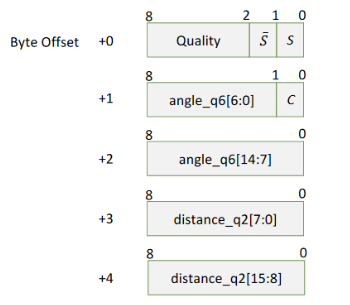
\includegraphics[width=.6\linewidth]{SYNTHESIS/protocolbreakdown.png}
		\caption{Protocol Breakdown}
		\label{fig:protocolbreakdown}
	\end{figure}
	
	So, for example, the first 6 bits of the first returned byte is used to store the scan's quality value. The idea behind the initial map processing software was to start at the beginning of the file containing binary scan data, then iterate through it by taking chunks of bits and storing them in variables.
	
	\begin{lstlisting}
	# Read in the bits according to the LIDAR response structure
	quality = f.read(6)
	inverseStart = f.read(1)
	start = f.read(1)
	angle_first = f.read(7)
	checkbit = f.read(1)
	angle_second = f.read(8)
	distance = f.read(16)
	\end{lstlisting}
	One small additional tweak that needed to be made was joining the first and second angle chunks together to form the full value.
	
	\begin{lstlisting}
	# Append the angle_q6 bits
	angle = (b"".join([angle_first, angle_second]))
	\end{lstlisting}
	
	The protocol documentation states that these aren't the true values however. The actual angle value is the binary value divided by 64 degrees, and the actual distance value is the binary value divided by 4 millimeters.
	
	\begin{lstlisting}
	# Turn binary into decimal
	# 'Actual heading = angle_q6/64.0 Degree'
	angle = (int(angle, 2) / 64.0)
	# 'Actual Distance = distance_q2/4.0 mm'
	distance = (int(distance, 2) / 4.0)/100
	\end{lstlisting}
	These points were then turned into mappable X and Y values. Despite all of this, none of this worked as intended. The produced maps made no logical sense, fig \ref{fig:failedmap} shows a map produced via this method from scans obtained from the inside of a rectangular box.
	\begin{figure}[ht]
		\centering
		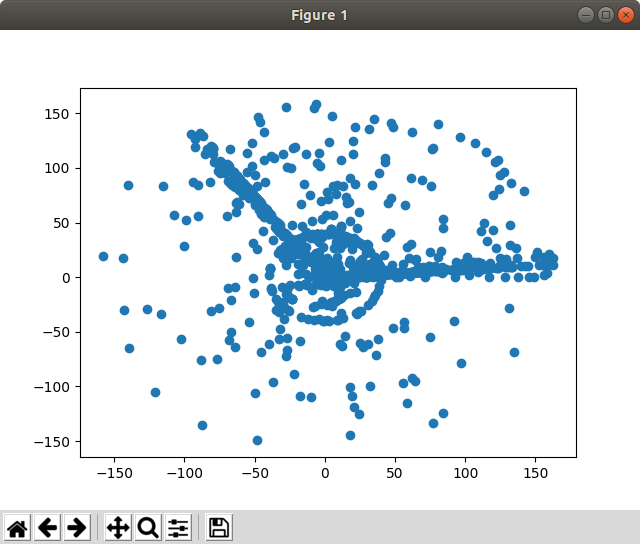
\includegraphics[width=.6\linewidth]{SYNTHESIS/failedmap.png}
		\caption{Resulting map of a box}
		\label{fig:failedmap}
	\end{figure}
	
	The generated values were printed, and it was observed that every now and then angles would be impossible values above 360. After all of this it was decided to go back to the drawing board and attempt to get the SDK working again since using the protocol was rapidly leading nowhere and burning time. Searching around on the mbed website stumbled across a robotic program that made use of a similar LIDAR system by SLAMTEC. The SDK in use there was a modified version that seemed to work fine with embedded systems, but still had all the necessary open licensing. This SDK was tested with the program and compiled fine, and is what was used to ultimately implement the robot's observational capability.
	
	\section{Scanning Inconsistency}
	One problem that repeatedly impeded development was the inconsistency in the LIDAR's scanning behaviour. Once development began to focus on writing real observational data into a buffer rather than filling it with dummy data just to prove the process, a number of issues began to crop up.
	
	The first was that occasionally entire batches of scan data would be zeroes. Every single angle and distance measurement would be a 0.0000000 float, with no changes to the buffer size making a difference. Pin connections were double checked and sometimes simply removed and plugged in again but then the scan straight after would result in the same thing happening. The troubleshooting section of the RPLIDAR A1M8 documentation was consulted. One suggestion was that the LIDAR core worked better once it had warmed up, and that it should be left spinning for a minute or so before it begins taking measurements. A simple task delay was introduced for 2 minutes before the main program loop began, but this issue would still come up sometimes. The quickest fix was generally to just recompile the program, and the issue would more often than not seemingly go away.